\section{Evaluation}
\label{sec:eval}

In this section, our benchmark is the CNN/Daily
Mail~\footnote{https://cs.nyu.edu/˜kcho/DMQA/}
dataset \cite{HermannKGEKSB15,NallapatiZSGX16,SeeLM17},
consisting of single source documents with multi-sentence summaries.
The dataset includes 286,817 training pairs,
13,368 validation pairs and 11,487 test pairs.
%\tabref{table:cnn} shows an example pair from training data.
We follow the pre-processing step as See 
 \shortcite{SeeLM17},
complementing the text slots with named entities.
We show an example of such pairs in \tabref{tab:gold_a}.

We compare our length constrained summarization model with
the basic CNN seq2seq model without length control and the state-of-the-art
length controllable summarization model \cite{abs-1711-05217}
in the following two experiments.\footnote{All generated summaries in this section
can be downloaded from \url{http://202.120.38.146/sumlen}.} Following Fan \shortcite{abs-1711-05217},
we distribute the dataset into a set of buckets which denote different lengths.
Each bucket is disjoint with other buckets and contains roughly
the equal number of documents.
The distribution is shown in \figref{fig:buckets}.

\begin{figure}[th!]
\centering
\scalebox{0.55}{\includegraphics[width=1.0\columnwidth]{data_LRC.eps}}
\caption{The buckets distribution for LRC} \label{fig:buckets}
\end{figure}

All the competing methods
have three flavors: {\em free length}, {\em truncated} and {\em exact}.
In the free length version(Free), given the desired length $N$,
each method generates summaries naturally until
an EOS is generated. And we limit the length of generated 
summaries to 100.~\footnote{The maximum length of summaries in CNN/DailyMail dataset is 94.}
This version usually generates
more complete and fluent summaries.
In the truncated version(Trunc), each method artificially
inserts an EOS if EOS is not generated in the first $N$ steps.
In the exact version(Exact), each method
generates $N$ non-EOS tokens and insert an EOS after the $N$-th token.
The purpose of the Free version is to evaluate the method's ability to
generate summaries of desired length; the purpose of the other
two versions is to enable fair comparison of the summaries in terms of
their content given that the summaries are of equal length. 
%Whereas the performance of Trunc and Exact version shows the effectiveness 
%of a method to generate readable summaries with the length constraint.

Next, we introduce the evaluation metrics in the following experiments:
\begin{enumerate}
\item \textit{ROUGE} scores(F1 score) of the produced
summaries, including ROUGE-1(R-1), ROUGE-2(R-2) and
ROUGE-L(R-L)~\cite{rouge-a-package-for-automatic-evaluation-of-summaries}.

\item \textit{Variance} of the summary lengths against
the desired length $len$;
%The variance is computed as following:
\begin{equation}
var = 0.001 * \frac{1}{n}\sum_{i=0}^{n} |l_i - len|^2, 
\end{equation}
where $n$ is the number of pairs in the dataset, and $l_i$ is the length of
the generated summary $i$. 
We introduce the variance as a metric to evaluate the
ability of exact control of the output length.

\item \textit{Similarity} between generated summaries
and their corresponding reference summaries.
%For length range $(l, r]$, we define the length error of the $i$-th pair as follows:
%\begin{equation}
%e_i = max\{0, max\{(r-x_i), (x_i-l)\}-R\},
%\end{equation}
%where $R$ is the range length (i.e. $r-l$) and $x_i$ denotes the actual length of
%the generated summary.
%We include the similarity metric because, when the desired length is very different
%from the gold length, the ROUGE scores may not reflect the true quality of the
%generated summaries. \KZ{We compute the similarity by ...}
\end{enumerate}

We leverage GloVe ~\footnote{https://nlp.stanford.edu/projects/glove/.}  
to capture the semantics of documents and summaries
and compute their semantic similarity (cosine similarity) to
measure the quality of the generated summary.
% More specifically, the similarity is computed as following:
\begin{equation}
sim = \frac{1}{n}\sum_{i=0}^{n} \frac{y_{i}\cdot y^{'}_{i}}{||y_{i}||\times ||y^{'}_{i}||}
\end{equation}
where $N$ is the dimension of the word vector. $y_i$ is
the reference summary $i$ and $y^{'}_{i}$ is the corresponding generated summary $i$. 
%We include similarity as a metric to evaluate the
%ability of semantic generation of the output.

%ROUGE scores tend to favor longer summaries.
%Therefore, we compute ROUGE scores
%on both the naturally produced summary (without truncation)
%and the summary after truncating
%to the desired length or the max length of a length range.


\subsection{Experimental Setup}
In the following experiments, 
all the competing models have 8 convolutional layers in
both encoder and decoder parts with kernel width as 3.
For each convolutional layer, 
we set the hidden size as 512 and the embedding size as 256.
To alleviate the overfitting problem,
we add the dropout ($p=0.2$) layer for 
all convolutional layers and fully connected layers.

%Following Gehring et al. 
%\shortcite{gehring2017convs2s,abs-1711-05217},
To optimize the proposed model,
we use Nesterov's
accelerated gradient method \cite{SutskeverMDH13} with gradient clipping 0.1 \cite{PascanuMB13}, momentum 0.99,
and learning rate 0.2.
We terminate the training process when the learning rate drops below $10e$-$5$.
We set beam size as 5 for the beam search algorithm in the testing step.
%For testing, we use beam search algorithm with the beam size 5.
%
%For length control model without penalty, we distribute the training set into a set of buckets which denote different length range. Each buchets does not overlap with other buckets and contains roughly an equal number of documents. For
%

\subsection{Experiment 1: Gold Summary Lengths}
\label{sec:exp1}

%In this part, we design different experiments to compare our models with basic model (CNN) and state of art model\citep{abs-1711-05217}.

In the first experiment, for each test document-summary pair, we set the desired length as the length of the gold summary
and ask the competing methods to generate a summary
with the desired length for each document.
%As shown in \tabref{table:gold},
%we compare the proposed model (LC) with the basic model (CNN) and the
%state of the art model(Fan) \citep{abs-1711-05217} on ROUGE scores
%and \textit{similarity}.
%ROUGE scores has limits
%We propose the \textit{similarity} metric to measure the
%quality of generated summary on the perspective of semantic level.
%
%\tabref{table:ROUGE-automatically} shows the ROUGE score and variance
%for these models.
%The column $Prob.$ is the probability of the generated summaries which belong to the correct length or length range.
As shown in \tabref{table:gold}, the proposed model (LC)
%consistently 
outperforms the other models on all of the evaluation metrics.
The ROUGE score shows the effectiveness of this model.
Lower variance reflects better length control of the model.
Higher similarity reflects better quality of generated summaries from the semantic 
point of view.
%Furthermore, our models can generate better summaries which have the setting length.

\begin{table}[h]
	\small
	\centering
	\caption{Desired Length: Gold Summary Lengths}
	\label{table:gold}
	\begin{tabular}{lcccccccc}
		\hline
		\multicolumn{2}{c}{}                                                     & R-1 & R-2 & R-L & Var & Sim \\ \hline
		\multicolumn{1}{c|}{\multirow{3}{*}{Free}} &
		\multicolumn{1}{l|}{CNN} & 34.49 & 14.38 & 25.78 & 0.3465 & 0.9220 \\ \cline{2-7}
		\multicolumn{1}{c|}{}                        & \multicolumn{1}{l|}{Fan} & 34.53 & 14.40 & 25.78 & 0.3446 & 0.9216 \\ \cline{2-7}
		\multicolumn{1}{c|}{}                        & \multicolumn{1}{l|}{LC} & \bf 35.45 & \bf 14.50 & \bf 26.02 & \bf 0.0005 & \bf 0.9272\\ \cline{2-7}
        \hline
		\multicolumn{1}{c|}{\multirow{3}{*}{Trunc}} &
		\multicolumn{1}{l|}{CNN} & \bf 34.76 & \bf 14.53 & 26.00 & 0.3045 & 0.9201 \\ \cline{2-7}
		\multicolumn{1}{c|}{}                        & \multicolumn{1}{l|}{Fan} & 35.44 & 14.52 & 25.97 & 0.3031 & 0.9197 \\ \cline{2-7}
		\multicolumn{1}{c|}{}                        & \multicolumn{1}{l|}{LC} & 34.74 & 14.50 & \bf 26.02 & \bf 0.0002 & \bf 0.9268\\ \cline{2-7}
        \hline
		\multicolumn{1}{c|}{\multirow{3}{*}{Exact}} &
		\multicolumn{1}{l|}{CNN} & 35.39 & 14.43  & \bf 26.07 & 0.0 & 0.9249 \\ \cline{2-7}
		\multicolumn{1}{c|}{}                        & \multicolumn{1}{l|}{Fan} & 35.37 & 14.42 & 26.03 & 0.0 & 0.9246 \\ \cline{2-7}
		\multicolumn{1}{c|}{}                        & \multicolumn{1}{l|}{LC} & \bf 35.44 & \bf 14.50 & 26.02 & 0.0 & \bf 0.9268 \\ \cline{2-7}
		\hline
	\end{tabular}
\end{table}

The LC model achieves the highest ROUGE and similarity score
as well as the lowest variance
in both Free and Exact version,
which shows the effectiveness of LC for generating 
high quality summaries under certain length constraint. 
In the Trunc version, the LC model outperforms the other 
comparable models on all evaluation metrics
except for the ROUGE score.
%In the Free version and Exact version, the ROUGE score and similarity score of LC model is the highest,
%and the variance of LC model is lowest. It means that we can control generated summary length best
%without lossing sematic information. 
%In the Trunc vesion, LC model is still the best on variance evaluation and 
%similarity evalution except the ROUGE score. 
%Comparing ROUGE scores of each model on different versions, we can
%find that our score is stable. It means that LC model can generate summaries in desired length without using any
%auxiliary method of controlling length. 
Note that, the ROUGE scores of LC model are
very stable, indicating its effective length control.
As for the other two models, 
they have better ROUGE score on Trunc version. 
However, as the example shown in \tabref{table:gold_example}, 
we argue that the similarity score is more reasonable 
to measure the quality of generated summary 
for the Trunc version. 

\begin{table}[th!]
\begin{center}
\caption{Example summaries generated by
gold summary length.}
\label{table:gold_example}
\small
\subtable[Source document and reference summary with 36 tokens]{
        \label{tab:gold_a}
        \begin{tabular}{lclc}%{|p{7cm}|rl|}
        \hline \bf Source document \\
        \hline the last time \color{green}{frank jordan} \color{black}{spoke with his son,} \color{red} {louis jordan} 
		       \color{black}{was fishing on \textbf{a sailboat a few miles off the south}}\\
			   \textbf{carolina coast}. the next time ... more than two months had passed and the younger jordan was on a contrainer\\
			   ship 200 miles from north carolina, just \textbf{rescued from his disabled boat} .
			   ``\textbf{i thought i lost you},''the relieved\\ 
			   father said. louis jordan, 37, took his sailboat out 
			   in \textbf{late january} and \textbf{hadn't been heard from in 66 days} ... the\\
			   \color{red}{younger jordan} \color{black}{said
			   \textbf{he took his sailboat out to the gulf stream to find some better fishing} ... the boat capsized} \\
			   two more times before he was \textbf{rescued}, according to jordan.\\
		\hline \bf Reference summary \\
        \hline \color{red}{louis jordan} \color{black}{says his sailboat capsized three times . 
		       he \textbf{survived} by collecting  rainwater and eating raw fish .}\\
			   \color{green}{frank jordan} \color{black}{told cnn \textbf{his son} is n't an experienced sailor but has a strong will .}\\
		\hline
        \end{tabular}
        }
\qquad
\subtable[Free summary(29 tokens), Trunc summary(29 tokens) and Exact summary of CNN]{
        \label{tab:gold_b}
        %\begin{tabular}{lcccccccc}
	    \begin{tabular}{p{1.8em}<{\centering}p{1.8em}<{\centering}p{21.5em}|p{2.5em}<{\centering}p{2.5em}<{\centering}p{2.5em}<{\centering}p{2.5em}<{\centering}p{2.0em}<{\centering}p{2.0em}<{\centering}}%{|p{7cm}|rl|}
      	\hline
		\multicolumn{2}{c}{}& Summary & R & P & F & Var & Sim  \\ \hline
		\multicolumn{1}{c|}{\multirow{4}{*}{CNN}} &
		\multicolumn{1}{c|}{Free} & \tabincell{l}{\color{green}{frank jordan} 
		                                           \color{black}{\textbf{took his sailboat out to the gulf stream}} \\ 
												   \textbf{to find some better fishing} , jordan says . `` it took so \\
												   long , '' jordan says . \\
												   } 
		& 6.06 & 9.09 & 7.27 & 0.049 & 0.9217 \\ \cline{2-8}
		\multicolumn{1}{c|}{}                        & 
		\multicolumn{1}{c|}{Trunc} & \tabincell{l}{\color{green}{frank jordan} 
		                                           \color{black}{\textbf{took his sailboat out to the gulf stream}} \\ 
												   \textbf{to find some better fishing} , jordan says . `` it took so \\
												   long , '' jordan says . \\
												   } 
		& 6.06 & \bf 9.09 & 7.27 & 0.049 & 0.9217 \\ \cline{2-8}
		\multicolumn{1}{c|}{}                        & 
		\multicolumn{1}{c|}{Exact} & \tabincell{l}{\color{green}{frank jordan} 
		                                           \color{black}{\textbf{took his sailboat out to the gulf stream}}\\
		                                           \textbf{to find some better fishing} , jordan says . jordan says\\
												    he took his sailboat out to the gulf stream to find some \\
													better fishing .\\
													} 
		& 6.06 & \bf 6.25 & 6.15 & - & 0.9254 \\ \cline{2-8}
        \hline
        \end{tabular}
        }
\qquad
\subtable[Free summary(50 tokens), Trunc summary(36 tokens) and Exact summary of Fan]{
        \label{tab:gold_c}
        %\begin{tabular}{lccccccc}
	    \begin{tabular}{p{1.8em}<{\centering}p{1.8em}<{\centering}p{21.5em}|p{2.5em}<{\centering}p{2.5em}<{\centering}p{2.5em}<{\centering}p{2.5em}<{\centering}p{2.0em}<{\centering}p{2.0em}<{\centering}}%{|p{7cm}|rl|}
      	\hline
		\multicolumn{2}{c}{}& Summary & R & P & F & Var & Sim  \\ \hline
		\multicolumn{1}{c|}{\multirow{4}{*}{Fan}} &
		\multicolumn{1}{c|}{Free} & \tabincell{l}{\color{green}{frank jordan}
		                                          \color{black}{\textbf{took his sailboat out to the gulf stream}} \\
		                                           \textbf{to find some better fishing .} jordan says he took his \\ 
												   sailboat out to the gulf stream to find some better \\
												   fishing . jordan says he took his sailboat out to the \\
												   gulf stream to find some better fishing .\\
		                                          }  
		& 6.06 & \bf 4.35 & 5.06 & 0.196 & 0.9215 \\ \cline{2-8}
		\multicolumn{1}{c|}{} & 
		\multicolumn{1}{c|}{Trunc} & \tabincell{l}{\color{green}{frank jordan}
		                                           \color{black}{took his sailboat out to the gulf stream} \\
		                                            to find some better fishing . \textbf{his son} , 
													\color{red}{louis jordan}\\ 
													\textbf{took his sailboat out to the gulf stream to find some} \\
													\textbf{better fishing .}\\
		                                           } 
		& 12.12 & \bf 12.90 & 12.50 & 0.0 & 0.9194\\ \cline{2-8}
		\multicolumn{1}{c|}{} & 
		\multicolumn{1}{c|}{Exact} & \tabincell{l}{\color{green}{frank jordan}
		                                           \color{black}{took his sailboat out to the gulf stream} \\
		                                           to find some better fishing . \textbf{his son} , 
												   \color{red}{louis jordan}\\ 
												   \textbf{took his sailboat out to the gulf stream to find some} \\
												   \textbf{better fishing .}\\
		                                           } 
		& 12.12 & 12.90 & 12.50 & - & 0.9194\\ \cline{2-8}
        \hline
        \end{tabular}
        }
\qquad
\subtable[Free summary(36 tokens), Trunc summary(36 tokens) and Exact summary of LC(ours)]{
        \label{tab:gold_d}
        %\begin{tabular}{lccccccc}
	    \begin{tabular}{p{1.8em}<{\centering}p{1.8em}<{\centering}p{21.5em}|p{2.5em}<{\centering}p{2.5em}<{\centering}p{2.5em}<{\centering}p{2.5em}<{\centering}p{2.0em}<{\centering}p{2.0em}<{\centering}}%{|p{7cm}|rl|}
      	\hline
		\multicolumn{2}{c}{} & Summary & R & P & F & Var & Sim  \\ \hline
		\multicolumn{1}{c|}{\multirow{4}{*}{LC}} &
		\multicolumn{1}{c|}{Free} &  \tabincell{l}{\color{red}{louis jordan} 
		                                            \color{black}{was on \textbf{a sailboat a few miles off the}}\\
		                                            \textbf{south carolina coast} . he \textbf{had n't been heard from }\\
													\textbf{in 66 days} when he was \textbf{rescued} . he was \textbf{rescued}\\
													\textbf{from his boat} .\\
		                                           }
		& 6.06 & 6.06 & 6.06 & 0.0 & \bf 0.9293 \\ \cline{2-8}
		\multicolumn{1}{c|}{}                        & 
		\multicolumn{1}{c|}{Trunc} &  \tabincell{l}{\color{red}{louis jordan} 
		                                            \color{black}{was on \textbf{a sailboat a few miles off the}}\\
		                                            \textbf{south carolina coast} . he \textbf{had n't been heard from }\\
													\textbf{in 66 days} when he was \textbf{rescued} . he was \textbf{rescued}\\
													\textbf{from his boat} .\\
		                                           }
		& 6.06 & 6.06 & 6.06 & 0.0 & \bf 0.9293 \\ \cline{2-8}
		\multicolumn{1}{c|}{}                        & 
		\multicolumn{1}{c|}{Exact} &  \tabincell{l}{\color{red}{louis jordan} 
		                                            \color{black}{was on \textbf{a sailboat a few miles off the}}\\
		                                            \textbf{south carolina coast} . he \textbf{had n't been heard from }\\
													\textbf{in 66 days} when he was \textbf{rescued} . he was \textbf{rescued}\\
													\textbf{from his boat} .\\
		                                           }
		& 6.06 & 6.06 & 6.06 & - & \bf 0.9293 \\ \cline{2-8}
        \hline
        \end{tabular}
        }
\end{center}
\end{table}

The ROUGE score consists of Recall(R), Precision(P) and F1-measure(F). 
The summary tends to achieve a better ROUGE score 
when the length of generated summary is slightly shorter than 
the desired length.
%, since the tokens generated in the first are usually more preciser.
%However, such ROUGE score can not 
%reflect the semantic information of the summary.
%although it has the problem of the lack of 
%the semantic information.
As shown in \tabref{tab:gold_b}, 
the CNN model has the same R score 
as LC model and has a higher P score than LC model because of its slightly
shorter length.  
We can see that the CNN model achieve a higher F score even its generated summary is not good. 
Moreover, for the basic model,
the generated summary always repeat the sentences
when the length of generated summary is longer than the desired length.
As shown in \tabref{tab:gold_c}, 
the P score of its Trunc version would be improved
by a large margin.
%As shown in \tabref{tab:gold_c}, its P score grows up by a large margin from Free version to Trunc version. 
Thus, the ROUGE score for the Trunc version shows a bias for 
the models with worse length control.
%So the Trunc version is advantageous to the model which can 
%not control the summary length well.
The generated summaries of the LC model in \tabref{tab:gold_d}, which capture the semantics of the reference summary and 
satisfy the constraint length very well,
are better than the other two models even with a slightly lower ROUGE score.
%contains the most information of source documents and satisfies the gold length.
%We can see that the generated summary of LC model is
%better than other two but our ROUGE score is slightly lower. 

The abstractive 
summarization attempts to reproduce the semantics 
and topics of original text
by paraphrasing, which tends to introduce fresh words and phrases into the summaries and is considered
more favorable. 
This causes the generated summary not to match the target 
summary word by word and gets a lower ROUGE score.
The topic of this example is that Louis Jordan ,who is the son of Frank Jordan, 
got lost during sailing and was finally rescued from his boat. 
Our model generates the summary with correct
information, but other two models get the Louis Jordan and Frank Jordan mixed up.
%Therefore, LC model still gets the highest similarity score on three version when our ROUGE score
%is not the best. 
Therefore, we argue that
the ROUGE score has limitations in evaluating 
abstractive summarization methods.
To ameliorate such limitation, 
we introduce the similarity metric which reflects the semantic information of the 
generated summary, especially in Exact version which can almost ignore the 
impact of different length.
We can see that the LC model achieves the highest similarity scores on
all three versions.

\subsection{Experiment 2: Arbitrary Lengths}
In the second experiment, we ask the methods to generate
summaries with arbitrary lengths. 
We report the results of all three methods with five arbitrary lengths: 10, 30, 50, 70 and 90.
%We test the models on several arbitrary desired lengths:
%10, 30, 50, 70 and 90.
%have different border in the same distance. And (0,10],(0,20] and (0,30] have different distance of range.
%Our length range control methods can handle point lengths by setting
%both the min and max value of the input range to be the desired length.
We show the performance of each model with different
length constraints in \tabref{table:arbi}, \figref{fig:Sim} and \figref{fig:var}.
The basic CNN model has the same ROUGE scores in the Free version since it cannot control the length of generated 
summaries on its own.
%, we the summaries it produces are automatically truncated at the max of the desired
%length
%length range or the desired length.
For \cite{abs-1711-05217}, the desired length is mapped to
the model's predefined fixed length range(s) that {\em contains}
the desired length before it produce its summaries. For example,
the desired length $10$ is mapped to the first bucket $(0, 33]$.
The ROUGE scores of Fan model in Free 10 and Free 30 are the same.
To demonstrate the effectiveness of LC model and
 further illustrate the results,
we show an example summary generated by LC(Free) model 
with different lengths as a representative. 
%As is shown in \tabref{tab:example}, the summaries with different length have a high quality
%on both sematics and length controlling. 
As shown in \tabref{tab:example}, when the desired length (e.g., 10) is
very different from the length of the reference summary, the ROUGE score
may not be good even though the generated summary matches the reference
quite well semantically. 

\begin{table}[th!]
	\centering
	\small
	\caption{Generated summaries of LC (Free) model}
	\label{tab:example}
	\begin{tabular}{|c|l}
	\hline
	\multicolumn{1}{c|}{\multirow{1}{*}{10}} &
	\tabincell{l}{
	    the \color{red}{younger jordan} \color{black}{was \textbf{rescued from his disabled boat}} .\\
	} 
	\\ \hline
	\multicolumn{1}{c|}{\multirow{1}{*}{30}} &
	\tabincell{l}{
	    \color{red}{louis jordan} \color{black}{was \textbf{rescued from his disabled boat} . 
		he \textbf{had n't been heard from in 66 days in }}\\
		\textbf{late january} . he was rescued from his disabled boat . \\   
	} 
	\\ \hline
	\multicolumn{1}{c|}{\multirow{1}{*}{50}} &
	%\multicolumn{1}{c|}{Free} & 
	\tabincell{l}{ 
	   `` \textbf{i thought i lost you} , '' jordan says . the \color{red}{younger jordan} 
	   \color{black}{was on \textbf{a sailboat a few}} \\
	   \textbf{miles off the south carolina coast} . `` i thought i lost you , '' jordan tells \textbf{his son} . jordan\\
	   says he was grateful to the people .\\
	} 
	\\ \hline
\end{tabular}
\end{table}

In this experiment, 
the desired length is fixed for all the documents which is independent from 
the corresponding lengths of reference summaries
%Besides, we can set different lengths to generation model for one source document. This makes the
such that the generated summaries may include more versatile 
words and phrases different from the reference summaries.
Thus, the similarity score is more reasonable for the evaluation than 
the ROUGE score.
As shown in \figref{fig:Sim} and \figref{fig:var}, 
the LC model achieves the lowest variance and highest similarity score
except the length of $10$ and $30$ in the Free version.
There is only 5\% of testing data with the length of reference summary shorter 
than 30. 
Since the effectiveness of the LC model on length control,
the lengths of generated summaries from LC model are 
usually much shorter than those from the other models and 
the length of corresponding reference summaries
when we set the desired length as 10 or 30.
This leads to a relative lower similarity score.

%In , we can see that no one model can always be the best in the ROUGE score.
%So the ROUGE score can not reflect the quality of generated summary in this experiment. 
%Actually, the experiment 1 is the special case of experiment 2. 
%The problem (CNN and Fan 
%can get advantage in the Trunc version) in the 
%experiment 1 can also appears in experiment 2. 
%The repetition of the basic CNN seq2seq
%is still existed.
%Besides, we can set different lengths to generation model for one source document. This makes the
%generated summaries contain more words or phrase different from the reference summary.

%when the desired length is $10$, it is hard to match the reference summary
%for generated summaries. 
%However, the generated summaries can not match the reference summary
%well. 
%As the highest ROUGE scores are scattered in three models, 
%we should consider the similarity and variance. 
%It means LC model can effectively control the length of generated summary. 
%In the \figref{fig:Sim}, 
%the similarity score of LC model are better than others excepts length $10$ and $30$ in the Free version. 
%The reason is that the length of summaries generated by LC model is very close
%to $10$ or $30$. The generated summaries of other two models have longer length than $10$ 
%or $30$. The cosine similarity score tends to be small when the summary is too short.
%So this is a normal phenomenon.
%can generate summaries with setting length constraint.
%\tabref{ROUGE-maxlendiff}
% shows ROUGE score in different range with setting the max length
%of generated summaries as the max value in the range.
%As \label{ROUGE-maxlendiff} shows that our models can generate better
%summaries with any length range.

%experiment 2
\begin{table}[th!]
	\centering
	\small
	\caption{Desired Length: 10, 30, 50, 70, 90}
	\label{table:arbi}
    \subtable[\textbf{Free} version]{
	    \begin{tabular}{p{1.8em}<{\centering}p{1.8em}<{\centering}p{1.8em}<{\centering}p{1.8em}<{\centering}p{1.8em}<{\centering}p{1.8em}<{\centering}p{1.8em}<{\centering}p{1.8em}<{\centering}p{1.8em}<{\centering}p{1.8em}<{\centering}p{1.8em}<{\centering}p{1.8em}<{\centering}p{1.8em}<{\centering}p{1.8em}<{\centering}p{1.8em}<{\centering}p{1.8em}<{\centering}}%{|p{7cm}|rl|}
		\hline
		\multirow{2}{*}{Free}&
		\multicolumn{3}{c}{10}&\multicolumn{3}{c}{30}&\multicolumn{3}{c}{50}&\multicolumn{3}{c}{70}&\multicolumn{3}{c}{90}\cr
		\cmidrule(lr){2-4} \cmidrule(lr){5-7} \cmidrule(lr){8-10} \cmidrule(lr){11-13} \cmidrule(lr){14-16}
		& CNN & Fan & LC & CNN & Fan & LC & CNN & Fan & LC & CNN & Fan & LC & CNN & Fan & LC \cr
		\hline
		R-1 & \bf34.49 & 34.28 & 19.03 & \bf34.49 & 34.28 & 32.26 & 34.49 & 34.60 & \bf34.71 & 34.49 & \bf34.65 & 33.83 & \bf34.49 & 30.56 & 32.17 \cr
		R-2 & \bf14.38 & 14.18 & 8.45  & \bf14.38 & 14.18 & 13.60 & 14.38 & \bf14.41 & 14.24 & 14.38 & \bf14.50 & 13.67 & \bf14.38 & 12.20 & 13.00 \cr
		R-L & \bf25.78 & 25.60 & 16.47 & \bf25.78 & 25.60 & 24.64 & 25.78 & \bf25.79 & 25.62 & 25.78 & \bf25.82 & 24.67 & \bf25.78 & 22.08 & 23.28 \cr
		\hline
        \end{tabular}
        }
     \subtable[\textbf{Trunc} version]{
	    \begin{tabular}{p{1.8em}<{\centering}p{1.8em}<{\centering}p{1.8em}<{\centering}p{1.8em}<{\centering}p{1.8em}<{\centering}p{1.8em}<{\centering}p{1.8em}<{\centering}p{1.8em}<{\centering}p{1.8em}<{\centering}p{1.8em}<{\centering}p{1.8em}<{\centering}p{1.8em}<{\centering}p{1.8em}<{\centering}p{1.8em}<{\centering}p{1.8em}<{\centering}p{1.8em}<{\centering}}%{|p{7cm}|rl|}
		\hline
		\multirow{2}{*}{Trunc}&
		\multicolumn{3}{c}{10}&\multicolumn{3}{c}{30}&\multicolumn{3}{c}{50}&\multicolumn{3}{c}{70}&\multicolumn{3}{c}{90}\cr
		\cmidrule(lr){2-4} \cmidrule(lr){5-7} \cmidrule(lr){8-10} \cmidrule(lr){11-13} \cmidrule(lr){14-16}
		& CNN & Fan & LC & CNN & Fan & LC & CNN & Fan & LC & CNN & Fan & LC & CNN & Fan & LC \cr
		\hline
		R-1 & \bf20.14 & 20.12 & 18.77 & 32.96 & \bf32.99 & 32.25 & 35.14 & 35.07 & \bf35.60 & 34.49 & \bf34.67 & 33.83 & 31.27 & \bf34.70 & 32.16 \cr
		R-2 & \bf9.27 & 9.22 & 8.31 & \bf14.06 & 14.04 & 13.60 & \bf14.46 & 14.40 & 14.30 & 14.38 & \bf14.50 & 13.67 & 12.40 & \bf14.55 & 13.00 \cr 
		R-L & \bf17.35 & 17.34 & 16.28 & \bf25.11 & 25.06 & 24.62 & \bf26.09 & 26.05 & 25.90 & 25.78 & \bf25.82 & 24.67 & 22.69 & \bf25.86 & 23.29 \cr
		\hline
        \end{tabular}
        }
     \subtable[\textbf{Exact} version]{
	    \begin{tabular}{p{1.8em}<{\centering}p{1.8em}<{\centering}p{1.8em}<{\centering}p{1.8em}<{\centering}p{1.8em}<{\centering}p{1.8em}<{\centering}p{1.8em}<{\centering}p{1.8em}<{\centering}p{1.8em}<{\centering}p{1.8em}<{\centering}p{1.8em}<{\centering}p{1.8em}<{\centering}p{1.8em}<{\centering}p{1.8em}<{\centering}p{1.8em}<{\centering}p{1.8em}<{\centering}}%{|p{7cm}|rl|}
		\hline
		\multirow{2}{*}{Exact}&
		\multicolumn{3}{c}{10}&\multicolumn{3}{c}{30}&\multicolumn{3}{c}{50}&\multicolumn{3}{c}{70}&\multicolumn{3}{c}{90}\cr
		\cmidrule(lr){2-4} \cmidrule(lr){5-7} \cmidrule(lr){8-10} \cmidrule(lr){11-13} \cmidrule(lr){14-16}
		& CNN & Fan & LC & CNN & Fan & LC & CNN & Fan & LC & CNN & Fan & LC & CNN & Fan & LC \cr
		\hline
		R-1 & \bf20.14 & 20.14 & 20.06 & \bf33.05 & 32.83 & 32.94 & 34.71 & 34.72 & \bf34.81 & 32.24 & 33.35 & \bf33.82 & 31.27 & 31.37 & \bf32.04 \cr
		R-2 & \bf9.27 & 9.23 & 9.23 & \bf14.08 & 13.79 & 14.00 & \bf14.78 & 14.17 & 14.23 & 13.33 & 13.39 & \bf13.59 & 12.41 & 12.47 & \bf12.86 \cr
		R-L & \bf17.36 & 17.36 & 17.30 & \bf25.15 & 24.87 & 25.02 & \bf25.65 & 25.63 & 25.60 & 24.31 & 24.35 & \bf24.56 & 22.69 & 22.76 & \bf23.14 \cr
		\hline
        \end{tabular}
        }
\end{table}

\begin{figure}[!htb]
  \subfigure[Similarity in Free version]{
  \label{fig:simF}
  %\begin{minipage}[t]{0.33textwidth}
    \centering
    \includegraphics[width=2in]{SimF.eps}
  %\end{minipage}
  }
  \subfigure[Similarity in Trunc version]{
  \label{fig:simT}
  %\begin{minipage}[t]{0.33\linewidth}
    \centering
    \includegraphics[width=2in]{SimT.eps}
  %\end{minipage}
  }
  \subfigure[Similarity in Exact version]{
  \label{fig:simE}
  %\begin{minipage}[t]{0.33\linewidth}
    \centering
    \includegraphics[width=2in]{SimE.eps}
  %\end{minipage}
  }
  \caption{Similarity of different length}
  \label{fig:Sim}
\end{figure}

\begin{figure}[!htb]
  \centering
  \subfigure[Variance in Free version]{
  \label{fig:varF}
  %\begin{minipage}[t]{0.5\linewidth}
    \centering
    \includegraphics[width=2in]{VarF.eps}
  %\end{minipage}%
  }
  \subfigure[Variance in Trunc version]{
  \label{fig:varT}
  %\begin{minipage}[t]{0.5\linewidth}
    \centering
    \includegraphics[width=2in]{VarT.eps}
  %\end{minipage}
  }
  \caption{Variance of different length}
  \label{fig:var}
\end{figure}
